\status{started}
\chapter{muEDM positron tracker}
\label{ch:muEDM:tracker}
\begin{refsection}
{\itshape This chapter is an in-depth study on the development of the scintillating fiber part of the muEDM positron tracker. 
We will skip some preliminary studies and we will start with the description of the positron tracker which was included in the proposal of the experiment submitted to PSI at the end of 2022. We will move to the simulations done after that and the current design of this detector.}

\status{started}
\section{Tracking $\Ae$ in muEDM}
    As already introduced in Ch.~\ref{ch:muEDM}, the muEDM experiment is based on the \textit{frozen spin} technique.
    For this purpose, it is cardinal to stop the muon in the right orbit. 
    After the muon has been stored, the careful calibration of the radial electric field will then change the $(g-2)$ precession, bringing it eventually to 0.
    At this point, the direction of the positron emission will be the relevant variable for the EDM search.
    These three steps require a way to track the outgoing $\Ae$ to assert the situation.
    Developing such a tracker in the muEDM environment is the challenge to which this chapter is dedicated.\\

    \noindent
    We will start by presenting the original detector design, which was developed to be complemented with silicon devices.

\section{Kinematics}
    \begin{table}[ht]
    \begin{tabular}{@{}p{2.2cm}p{2cm}ccc@{\hspace{10pt}}p{2cm}ccc@{}}
    \toprule
    \multicolumn{1}{c}{\multirow{2}{*}{Method}} & \multicolumn{4}{c}{Phase I} & \multicolumn{4}{c}{Phase II} \\ \cmidrule(l{2pt}r{10pt}){2-5} \cmidrule(l{2pt}r{2pt}){6-9} 
    \multicolumn{1}{c}{} & Threshold \scriptsize$\times \SI{68.9}{MeV}$ & \multicolumn{1}{c}{$\tilde \alpha$} & \multicolumn{1}{c}{$N_{e^+}/N_{\mu^+}$} & \multicolumn{1}{l}{FoM} & Threshold \scriptsize$\times \SI{140.2}{MeV}$ & \multicolumn{1}{c}{$\tilde \alpha$} & \multicolumn{1}{c}{$N_{e^+}/N_{\mu^+}$} & \multicolumn{1}{c}{FoM} \\ \midrule
    Simple & None & 0.166 & 1.0 & 0.166 & None & 0.166 & 1.0 & 0.166 \\ \midrule
    T-method & 0.596 & 0.348 & 0.384 & 0.216 & 0.183 & 0.195 & 0.835 & 0.178 \\ \midrule
    W-method \scriptsize(20 energy bins) & None & 0.251 & 1.0 & 0.251 & None & 0.183 & 1.0 & 0.183 \\
    W-method \scriptsize (20 energy bins) & 0.4 & 0.280 & 0.800 & 0.250 & 0.15 & 0.194 & 0.876 & 0.183 \\ \midrule
    W-method \scriptsize (20x20x20 bins) & None & 0.292 & 1.0 & 0.292 & None & 0.280 & 1.0 & 0.280 \\
    W-method \scriptsize (20x20x20 bins) & 0.4 & 0.326 & 0.800 & 0.291 & 0.15 & 0.299 & 0.876 & 0.280 \\ \bottomrule
    \end{tabular}
    \caption{Summary of analysis methods. The ratio $N_{e^+}/N_{\mu^+}$ is the fraction of detected positrons with respect to the total number of injected muons and $\tilde \alpha$ is the mean asymmetry above a threshold. The presented values are the theoretical maximum and do not include effects of multiple scattering of positrons or limited detector acceptance.}\label{tab:AnalysisMethods}
    \end{table}


\status{started}
\section{Design in the 2022 proposal}
    The kinematics of the $e^+$ coming from the decay is described in a Sec.~\ref{sec:StatSysEstimate}.
    From preliminary results, the resolutions required for the different studies are the following:
    \begin{description}
        \item[Momentum resolution] around a few MeV/c. This is mainly necessary for selection cuts on positrons with the desired asymmetry, which is momentum dependent, as discussed in Section \ref{sec:StatSysEstimate}.
        \item[Position resolution] around \SI{1}{mm}. This seems to be the necessary resolution for track fitting with the required uncertainties in the direction. 
        This result was achieved by geometric means, assuming that reliable timing information is not available. 
        \item[Timing resolution] less than \SI{1}{ns}. The \SI{28}{MeV/c} positron travels at \textit{c}, meaning that in the expected magnetic field a complete rotation takes $\gtrsim$ \SI{0.6}{ns} imposing a limit on the time resolution. 
    \end{description}
    
    To accomplish these requirements, we will implement a positron tracker based on scintillating fibers of \SI{250}{\micro\meter} size coupled to silicon photomultipliers~(SiPM). 
    This detector option allows for a fast, versatile, modular, and low-cost detector technology that is operational in magnetic fields and vacuum, the environment in which the muEDM measurement takes place.

    
\begin{figure}
    \centering
		\subfloat[]{\hspace{0.075\columnwidth}
    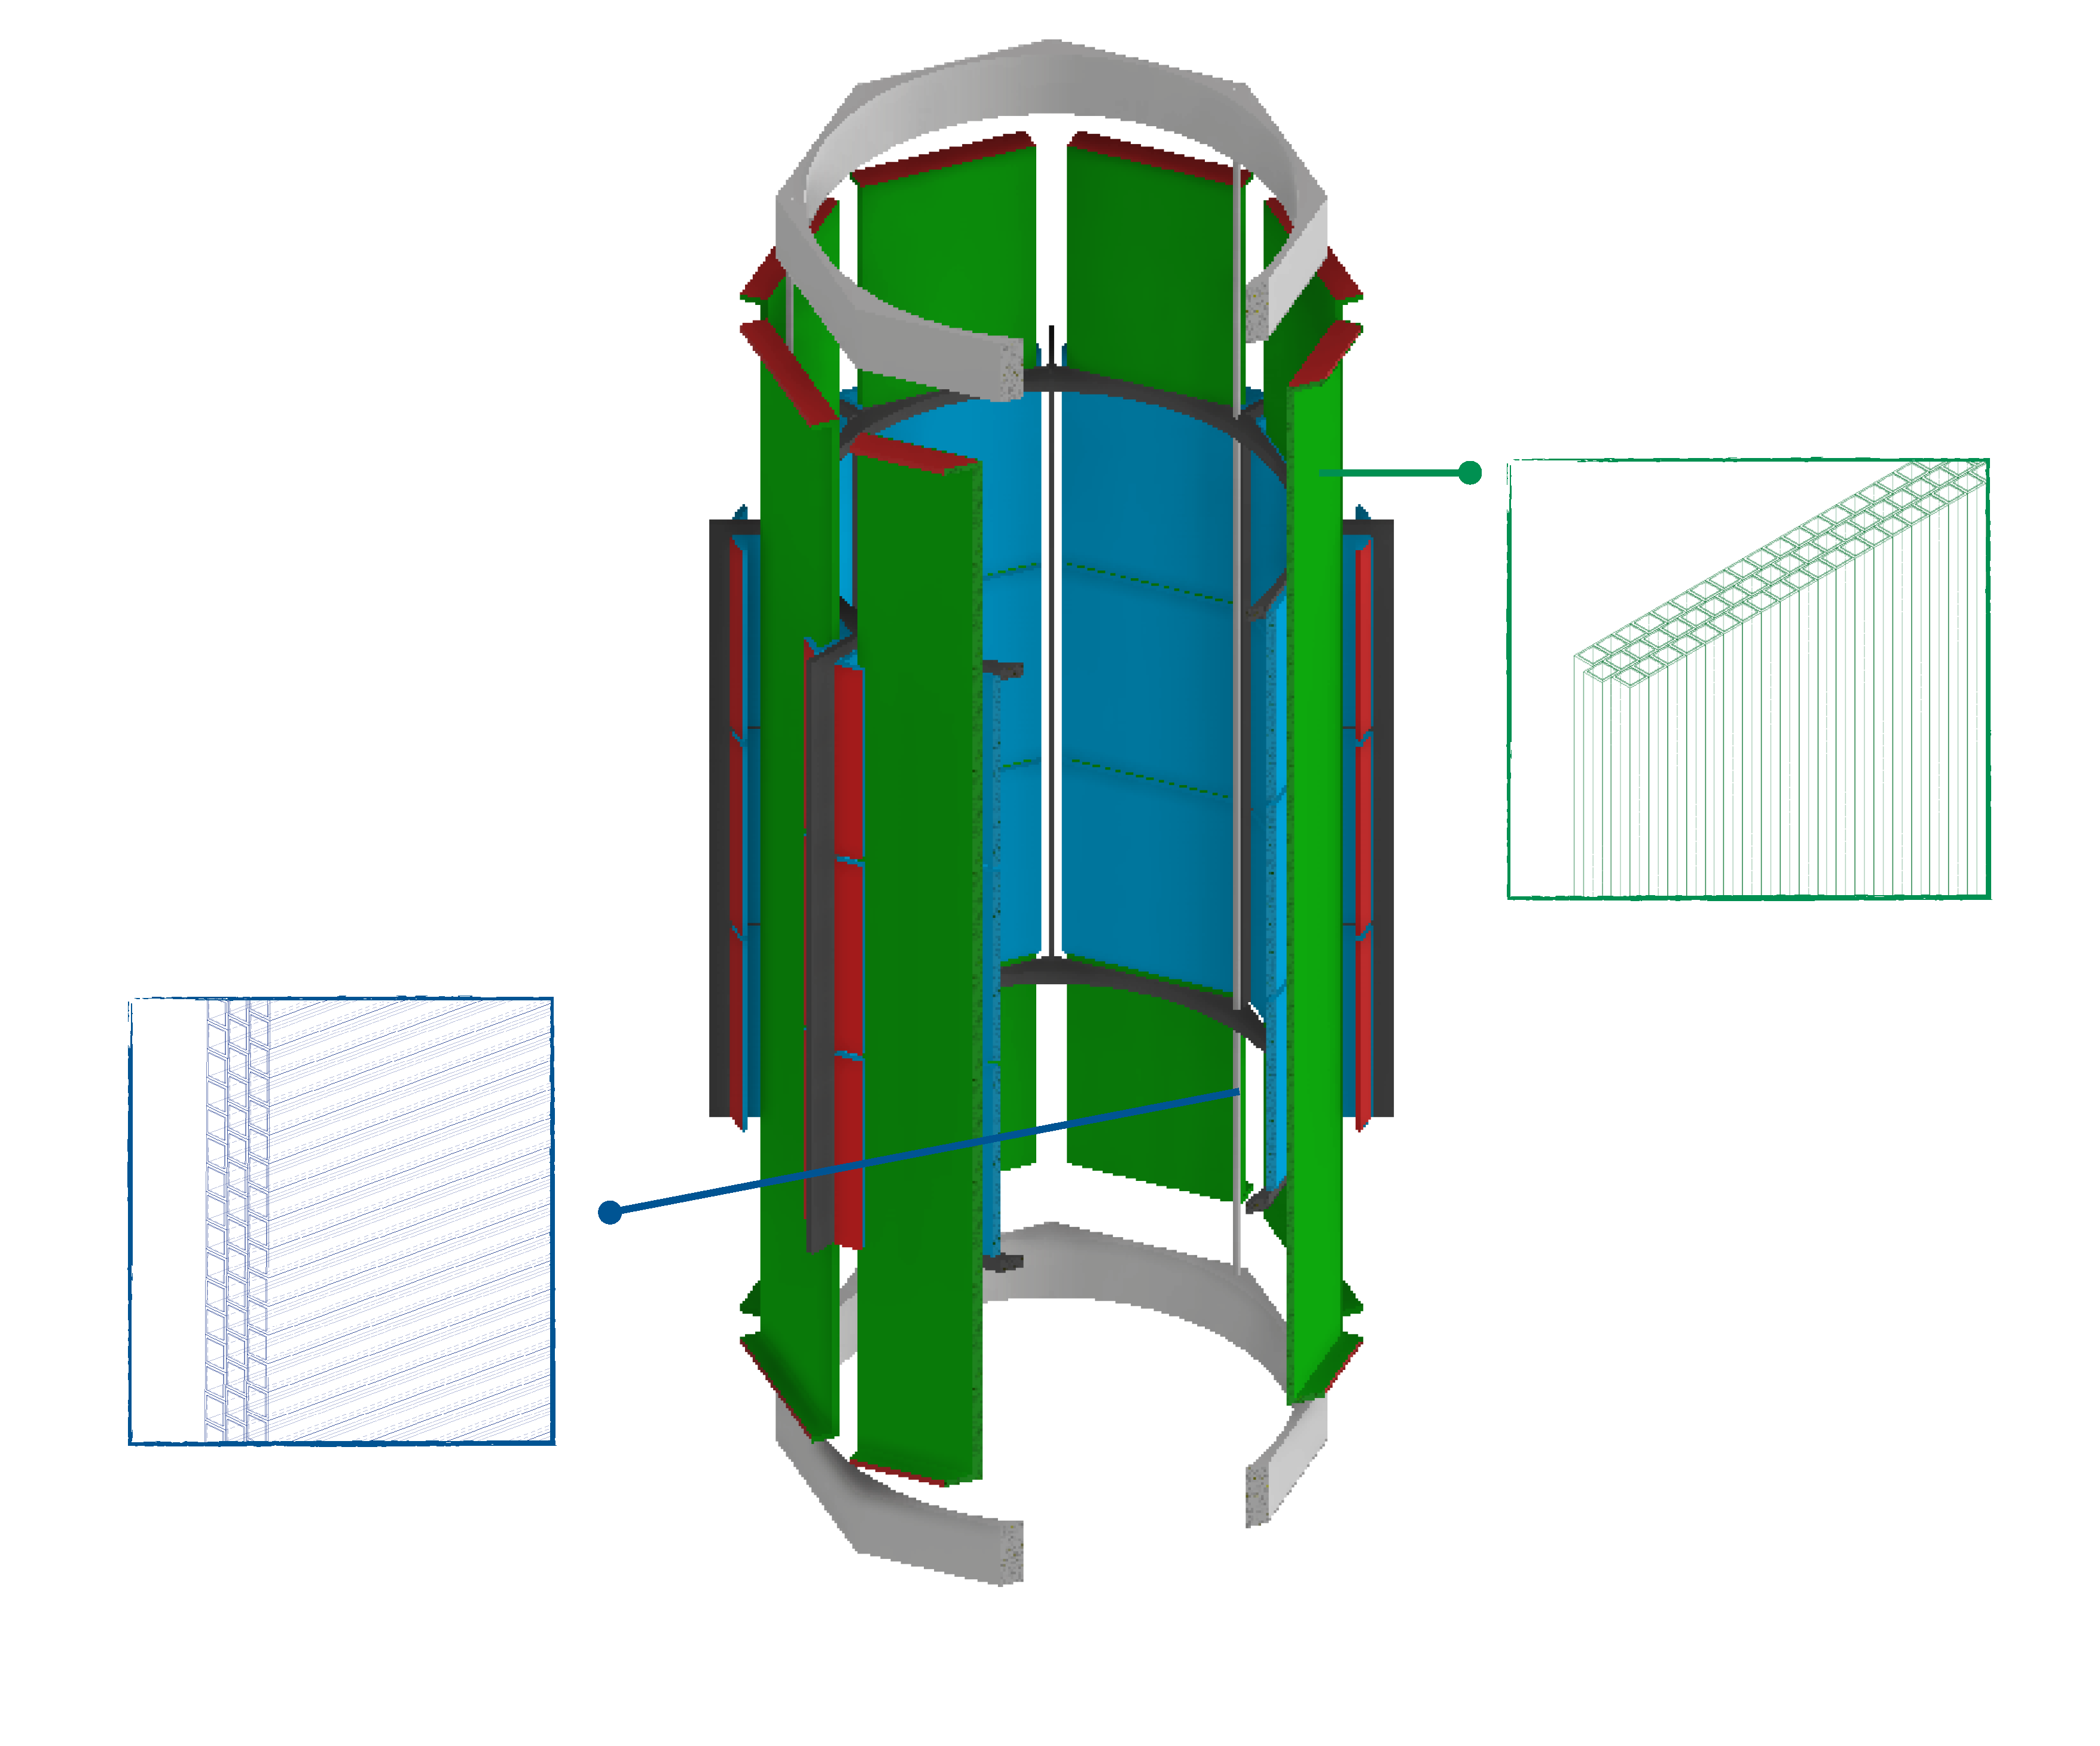
\includegraphics[width=0.55\columnwidth]{Figures/muEDM/Tracker/Assembly_muEDM_SciFi.png}
		}
		\hfill
		\subfloat[]{
		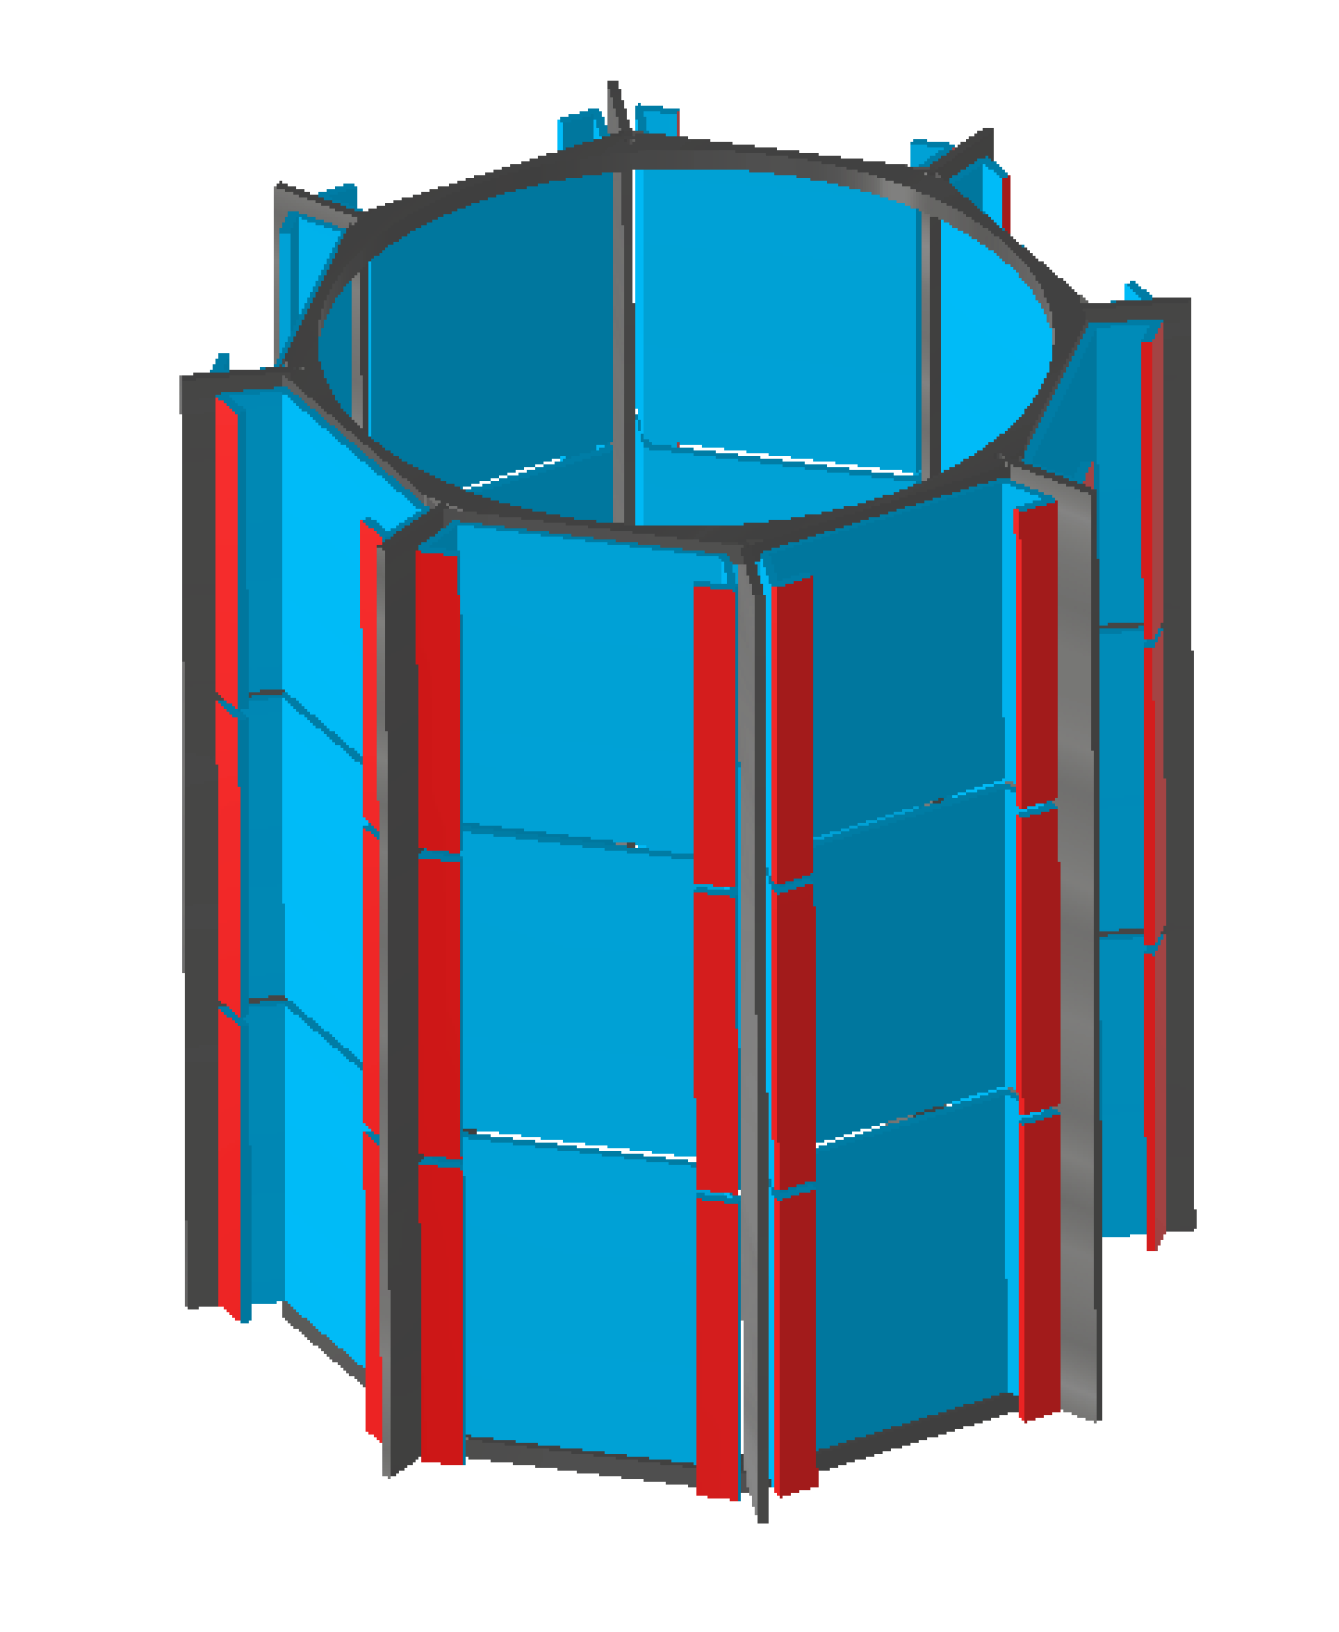
\includegraphics[width=0.25\columnwidth]{Figures/muEDM/Tracker/Assembly_InnerCup.png}
		\label{fig:SciFi_InnerDetector}
		\hspace{0.075\columnwidth}}
		\hfill
		\subfloat[]{
		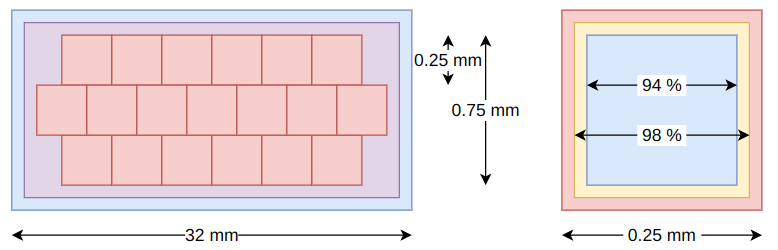
\includegraphics[width=0.5\textwidth]{Figures/muEDM/Tracker/SciFi.png}
		\label{fig:SciFi_MC}	}
    \caption{(a)~Sketch of the SciFi conceptual design. (b)~The inner part is made up of three barrels of scintillating fiber ribbons. Each barrel constitutes eight ribbons, with the fibers oriented transversely. This is the so-called SciFi transverse detector~(blue). The outer part is made of eight ribbons, with the fibers oriented longitudinally. This is the so-called SciFi longitudinal detector~(green). (c)~Left: Sketch of the layout of the fibers inside a SciFi ribbon. Right: A sketch of a fiber that comprises a \textit{core} and two \textit{claddings} of PMMA\@.}
    \label{fig:SciFi_ConceptualDesign}
\end{figure}

\status{started}
\subsection{The SciFi detector}
    The SciFi detector is designed to provide excellent tracking capacities for minimum-ionizing particles with a detector thickness below \SI{0.4}{\%}, a timing resolution better than \SI{1}{ns}, and a spatial resolution of \SI{1}{mm}, or probably better.
    Figure~\ref{fig:SciFi_ConceptualDesign} shows the first conceptual design of the detector. The tracker will be a compact detector made of several ribbons of \SI{250}{\micro m} scintillating fibers arranged in an inner~(transverse) and an outer~(longitudinal) detector.

The inner detector is made of a minimum of three barrels, extendable to five, of scintillating fiber ribbons. Each barrel is made of eight ribbons, with the fibers oriented transversely. This is the so-called SciFi transverse detector, as shown in Fig.~\ref{fig:SciFi_InnerDetector}, providing the necessary longitudinal resolution (up/down) to measure the EDM signal. In this detector, the fiber ribbons are polygonally shaped as shown by the blue elements in the figure. The red elements represent the photosensors. The optional outer detector is made of eight ribbons, with the fibers oriented longitudinally. Here, the ribbons have a parallelepipedal shape (green elements) with photosensors at both ends (red elements), as shown in Fig.~\ref{fig:SciFi_ConceptualDesign}. This is the SciFi longitudinal detector, which could complement the silicon strip detector discussed in the previous sections. Both detectors are arranged to cover a cylindrical surface, with the radius of the inner detector currently equal to \SI{50}{mm}.

Each ribbon has three layers of fibers, and these three layers are glued together in a staggered way, as sketched in Fig.~\ref{fig:SciFi_MC}. Each layer is made up of 128 \SI{250}{\micro m} square or round multiclad fibers. One layer has a width of approximately \SI{32}{mm} and a length of approximately \SI{200}{mm}. Each ribbon is read out at both ends by silicon photomultiplier (SiPM) arrays. Double-readout of each ribbon is essential for matching the experiment requirements. The amount of energy deposited in such a thin fiber by a mip is small ($\mathcal{O}(\SI{35}{keV})$) and, given the size of the detector, the relative light reaching the photosensor turns out to be equal to a few photons/fiber. 
To successfully collect these few photons with maximum efficiency and high dark noise rejection factor, a double readout scheme is foreseen, as well as extreme care in the coupling of the fibers to the photosensors.

\status{started}
\subsection{Geant4 simulation and performance}
For current simulations, fiber implementation is based on double-clad BCF20 Saint-Gobain scintillating fiber parameters\footnote{\url{https://www.crystals.saint-gobain.com/radiation-detection-scintillators/fibers}}.
The sketches of the fiber section and the ribbon are shown in Fig.~\ref{fig:SciFi_MC}.
Currently, we are performing simulations that include the interaction between radiation and matter using \textsc{GEANT4} physics processes. Complete photosensor readout and electronics will be implemented once all details of the detector are finalized. 
For these simulations, we assume an ideal readout scenario in which all photons that reach the ends of the fibers are detected and the exact position and timing of each photon are recorded. Additionally, each fiber is treated as a single detector element equivalent to a single fiber readout.

We are considering the possibility of merging multiple fibers into a single photosensor to reduce the number of channels required for the Data Acquisition System (DAQ) of the experiment. 
However, the performance of the resulting system may be compromised by the balance between the desired resolution and the number of available DAQ channels, as well as by the pixelation of the SiPMs. Despite this, the initial results of tests with a prototype ribbon using a fiber merging readout scheme under realistic conditions (including photosensor response, front-end electronics, and noise) show promising potential to meet muon EDM requirements, as described in Sec.~\ref{sec:SciFi_prototype}. These results were obtained using waveform analysis to extract the necessary information from the digitized data.

The expected performance of a single fiber ribbon for both position and timing resolution, where each \SI{250}{\micro m} fiber is read out independently, has been evaluated by dedicated studies. 
The first step is to study the characteristics and performance of a single ribbon. Having two impinging particles at the same time at a given distance, we can estimate the spatial resolution of this system.  Fig.~\ref{fig:geant4_position_resolution} shows an event with two particles separated by \SI{2}{mm}. Looking at the position of the generated photons, we can clearly distinguish the two hits, and the resolution is of the order of \SI{0.1}{mm}.

\begin{figure}
    \centering
    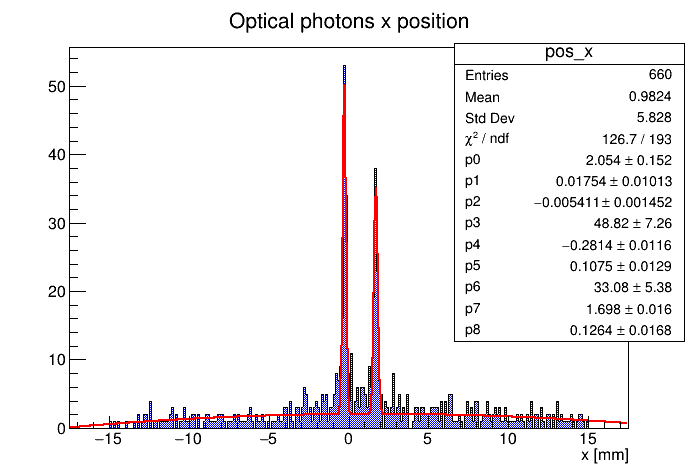
\includegraphics[width=0.5\textwidth]{Figures/muEDM/Tracker/2mm.png}
    \caption{Two particles impinging \SI{2}{mm} apart on the same ribbon. Using \SI{250}{\mum} fibers and having no pixelation on the readout, the spatial resolution is $\sigma\approx \SI{100}{\mum}$ (p5 and p8). This value was obtained with a fit to \textit{plo2+gauss+gauss} and with a bin width of \SI{125}{\mum} (half a fiber width).}
    \label{fig:geant4_position_resolution}
\end{figure}
    
In Fig.~\ref{fig:geant4_time}, the arrival time of the scintillating photons at the photosensor, generated by two consecutive particles, is shown. The position of the impinging particles is the same, but a different $\Delta t$ was set between them. Although the time resolution for a single particle is given by the rising edge of the distribution, much sharper than required $\sim \SI{1}{ns}$, the distribution itself is quite broad. This means that a particle that crosses at the exact same position within $\lesssim$ \SI{3}{ns} will induce a pile-up event. Note that here we neglect the shaping of the waveform, for which a width of \SIrange{10}{20}{ns} is expected. This is the time window within which a pile-up event could occur. The resulting distribution is still quite different from that of a single impinging particle, and this feature could be somewhat mitigated. On top of this, the probability of having no deflection due to multiple scattering on a full rotation is quite low: the spatial resolution will further mitigate this pile-up effect. 

\begin{figure}
    \centering
    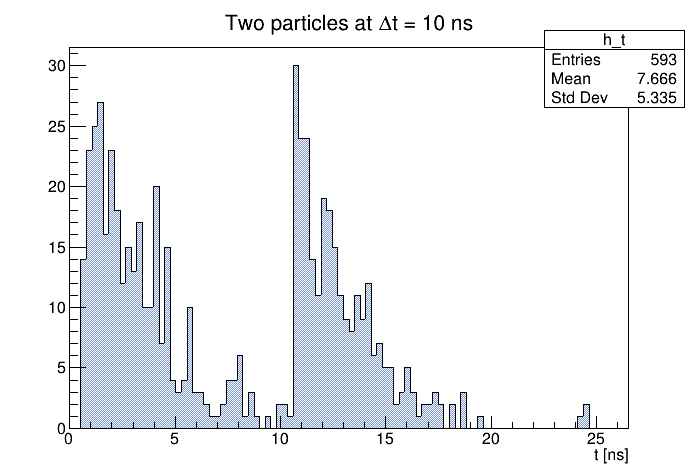
\includegraphics[width=0.32\textwidth]{Figures/muEDM/Tracker/10ns.png}
    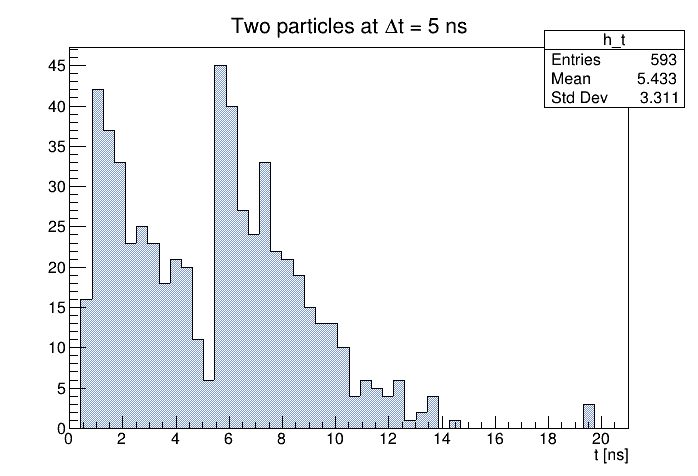
\includegraphics[width=0.32\textwidth]{Figures/muEDM/Tracker/5ns.png}
    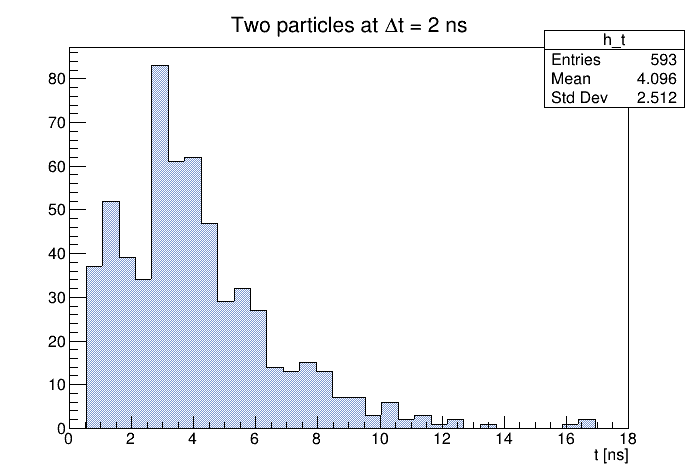
\includegraphics[width=0.32\textwidth]{Figures/muEDM/Tracker/2ns.png}
    \caption{In case of a particle impinging on the same position, the timing of the photon can be used to distinguish the two hits. For \SI{20}{cm} fibers, the limit seems to be \SIrange{3}{5}{ns}.}
    \label{fig:geant4_time}
\end{figure}

 \paragraph{Fibers and read-out} Aside from the specific geometry, the cardinal point is how to describe the fibers and their readout. 
        The fiber itself is simulated as a three-layer volume:
        \begin{outline}
            \1 Core: 
            \1 First cladding: PMMA
            \1 Second cladding: PMMA EMA
        \end{outline}
        The optical property of the surface between the different layers is specified with a G4OpticalSurface\footnote{The documentation can be found here: \href{https://apc.u-paris.fr/~franco/g4doxy/html/classG4OpticalSurface.html}{G4OpticalSurface}}.
        The readout is a somewhat simplified simulation of a SiPM (the same one used also for the different scintillators discussed in the previous chapter):
        \begin{outline}
            \1 Optical grease: to simulate the optical coupling of the SiPM to the fibers/scintillators
            \1 SiPM window: SiPMs have a Silicon resin window covering the active region
            \1 SiPM: The bulk of the SiPM is simulated as a simple block of silicon
        \end{outline}
        The idea of this readout is not to simulate the actual physical processes leading to an electric signal, but just to record the position and time of optical photons entering the system.


\vspace{2mm}
\paragraph{MuEDM geometry}~\\

Simulating the full geometry of our detector, including both the inner layer of transverse fibers and the outer layer of longitudinal fibers, and incorporating the effects of the magnetic field, leads to more complex events. An example is shown in Fig.~\ref{fig:geant4_B}. In this scenario, a single particle can pass through multiple layers, undergoing scattering and losing energy. The spatial information provided by both layers, as shown in Fig.~\ref{fig:geant4_position}, demonstrates that the positions of the hits on the transverse plane are relatively stable, probably due to the low material budget. On the contrary, the inner layer provides information about the longitudinal movement of the particle.

The incorporation of timing information for the transverse fibers results in the plot shown in Fig.~\ref{fig:geant4_time_pos}. This plot includes horizontal lines that represent the separation between different barrels. The relationship between transverse position and time provides additional information, although it can be more difficult to interpret. The resulting plots are shown in Fig.~\ref{fig:geant4_time_pos_transverse}.

\begin{figure}
    \centering
    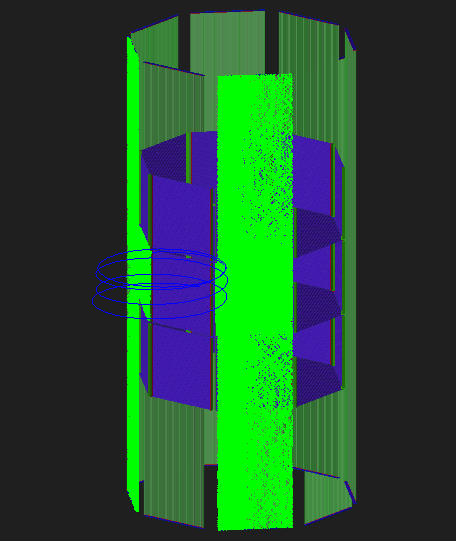
\includegraphics[width=0.5\textwidth]{Figures/muEDM/Tracker/muedm_scifi_B.png}
    \caption{An example of a \textsc{GEANT4} simulated event. In green the optical photons reflecting inside the fiber ribbons; in blue the trajectory of the positron. Keeping the same color scheme, the longitudinal SciFi is green while the transverse one is blue.
    }
    \label{fig:geant4_B}
\end{figure}

\begin{figure}
    \centering
    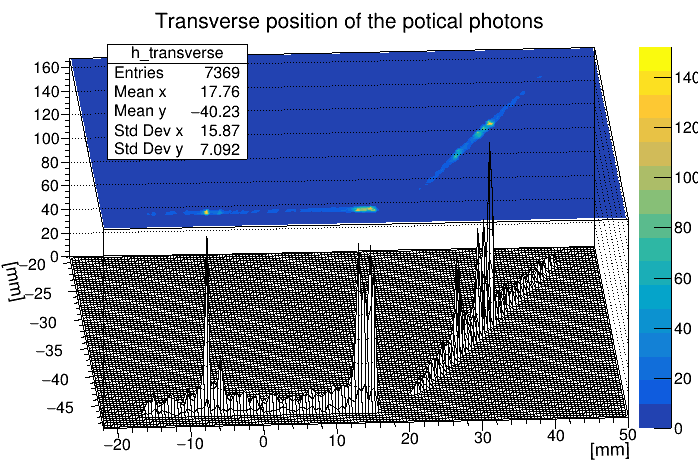
\includegraphics[width=0.45\textwidth]{Figures/muEDM/Tracker/fPosInXfPosInZ.png}
    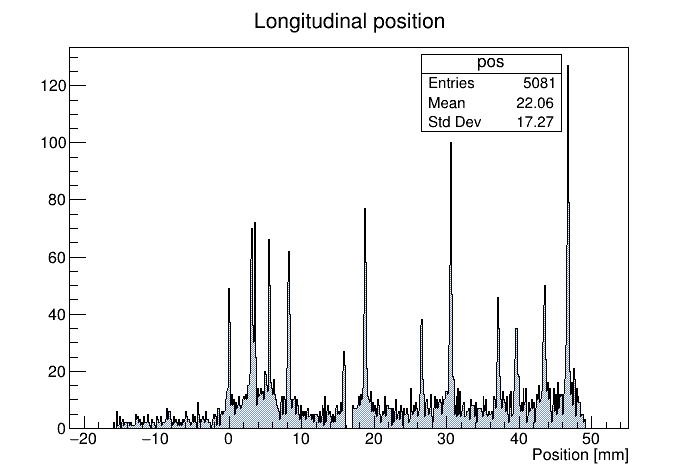
\includegraphics[width=0.45\textwidth]{Figures/muEDM/Tracker/fPosInY.png}
    \caption{Looking at the position for the photons arriving at the readout for both SciFi layers. 
}
    \label{fig:geant4_position}
\end{figure}

\begin{figure}
    \centering
    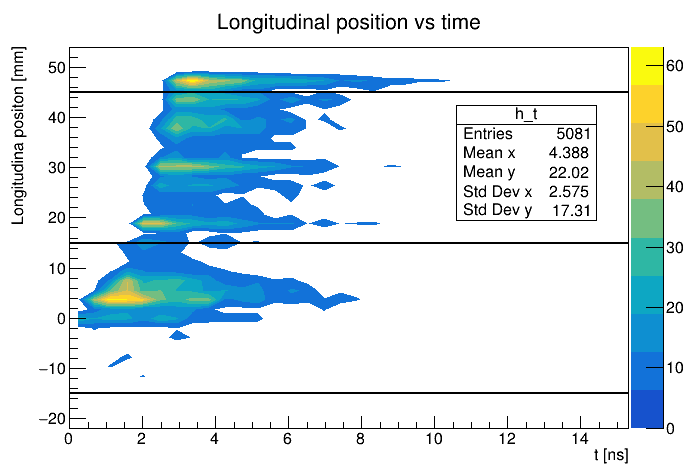
\includegraphics[width=0.5\textwidth]{Figures/muEDM/Tracker/fPosInYfTimeIn.png}
    \caption{Looking at the relationship between time and longitudinal position for the inner layer makes it possible to see if the particle is spiraling up or down.}
    \label{fig:geant4_time_pos}
\end{figure}

\begin{figure}
    \centering
    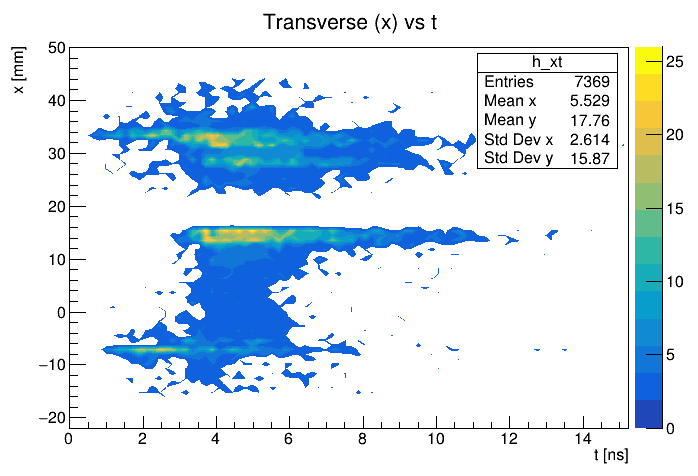
\includegraphics[width=0.45\textwidth]{Figures/muEDM/Tracker/fPosInXfTimeIn.png}
    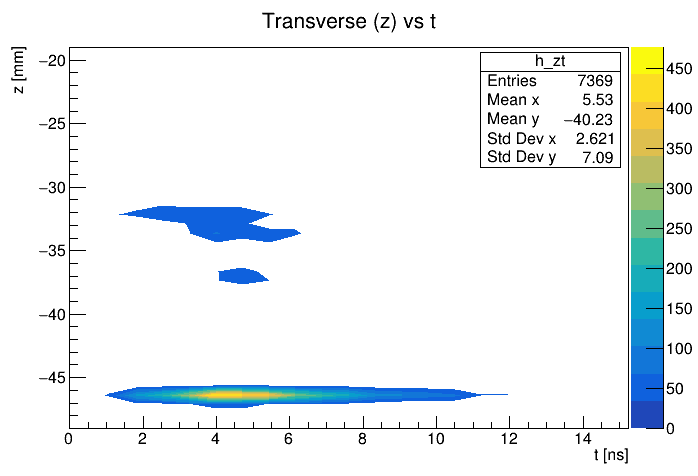
\includegraphics[width=0.45\textwidth]{Figures/muEDM/Tracker/fPosInZfTimeIn.png}
    \caption{The information from the joint use of transverse position and time, given by the outer layer, is more complex but nonetheless essential (and a unique feature of this detector) in understanding the particle trajectory.
}
    \label{fig:geant4_time_pos_transverse}
\end{figure}

\status{started}
\section{CHeT}
    The first step in developing and prototyping the geometry chosen in the previous paragraph is to understand the requirements for this sub-detector and how the prospected resolutions compare to these.
    This scintillating fiber tracker will be used for position tracking and in particular is going to be complemented by silicon strips. The crucial information this system needs to provide is the longitudinal position of the particle with a good resolution: $\delta \ell \lesssim \SI{1}{mm}$.

    \status{review}
    \subsection{Resoutions of crossed fibers ribbons}
        Let's consider a ribbon  $\SI{3}{cm}\times\SI{15}{cm}$ of squared fibers \SI{250}{\micro m} running vertically. Assuming a `perfect' readout, the resolution across the ribbon is given simply by the fibers' width while the resolution along the ribbon is extracted by reading the fibers on both sides. This second resolution is often quite worse than the previous. For practical purposes we will here assume $\delta_x = \SI{1}{mm};\ \delta_y = \SI{10}{mm}$.
        Rotating the ribbon by an angle $\theta$ changes the projection of the resolutions on the $\hat{x};\ \hat{y}$ axes and for this reason crossing two ribbons can improve the resolutions on the position of a crossing particle.
        When reading the ribbon on both sides the resolutions, as a function of $\theta$, are given by the smaller between the projection of the two intrinsic resolutions.  
        \begin{equation}
            \begin{cases}
            \dd x = min(\delta x \sec \theta;\ \delta y \csc \theta)\\
            \dd y = min(\delta x \csc \theta;\ \delta y \sec \theta)
            \end{cases}
        \end{equation}
        The relation between resolutions and the tilt angle is shown in fig. \ref{fig:CyFi:projected_dxdy}.  
        \begin{figure}
            \centering
            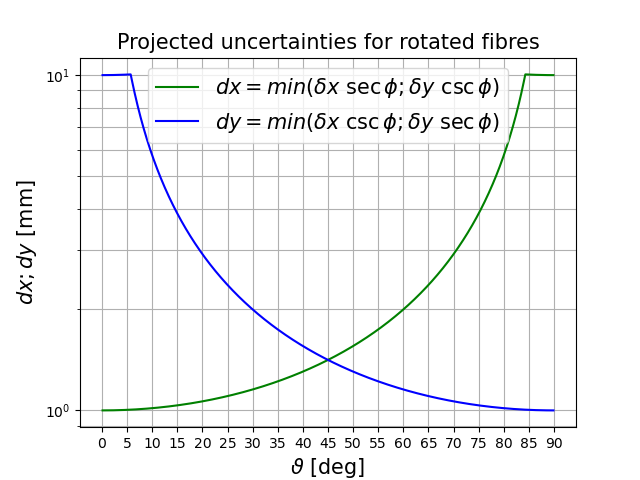
\includegraphics[width=\textwidth]{Figures/muEDM/CyFi/projected_dxdy.png}
            \caption{Projection along the $\hat{x};\ \hat{y}$ axes of the resolutions considering a ribbon of fibers rotated in different angles. The intrinsic resolutions are here assumed $\delta_x = \SI{1}{mm};\ \delta_y = \SI{10}{mm}$.}
            \label{fig:CyFi:projected_dxdy}
        \end{figure}

    \status{review}
    \subsection{Angle choices for the layers}
        When considering two layers the angles must be chosen to improve the overall resolution, which in practice means minimizing the uncertainty only on one axes per ribbon.
        Let's consider the different layouts in \ref{fig:CyFi:examples:a} and how they translate to resolutions in \ref{fig:CyFi:examples:b}.
        Clearly having the two ribbons at \SI{90}{\deg} along the axes is the best option but if we want to avoid having the readout on the plane of the muon orbit we need to consider less steep angles for the single ribbons.
        Options C and D are the possible solutions and, looking at the resolutions, D is actually the configuration minimizing the resolutions on both axes. 

    \status{started}
    \subsection{Cylindrical geometry}
        At this point is important to notice an additional constraint, given by the cylindrical geometry.
        If, instead of having planar ribbons, the fibers are woven into two concentric cylinders one needs to avoid having multiple crossings.
        If two fibers cross multiple times when both are scintillating the position of the impinging particle is ill-defined. There is a `real' crossing point but also additional `ghosts' hits.
        If we consider a two-layer system the requirement of having only one crossing point (i.d. no `ghosts') translates to having a difference in the number of turns $\lesssim1$. 
        In a cylindrical geometry the relation between the angle of the fibers and the number of turns completed, shown in Fig.~\ref{fig:CyFi:TurnsVsAngles}, is determined by the dimensions of the cylinder itself.
        At this point, we can plot the resolutions as a function of the angle of one of the layers keeping the angle for the second layer such as $\Delta T=1$. The results are in Fig.~\ref{fig:CyFi:projected_dxdy} while Fig.~\ref{fig:CyFi:angle} shows the difference in angle for the two layers.
        We will consider two concentric cylinders, the outer layer being the one with a shallower angle: this is intended to reduce the effect of multiple scattering on the longitudinal position.
        \begin{figure}
            \subfloat[Some possible orientation for two ribbons.]{
            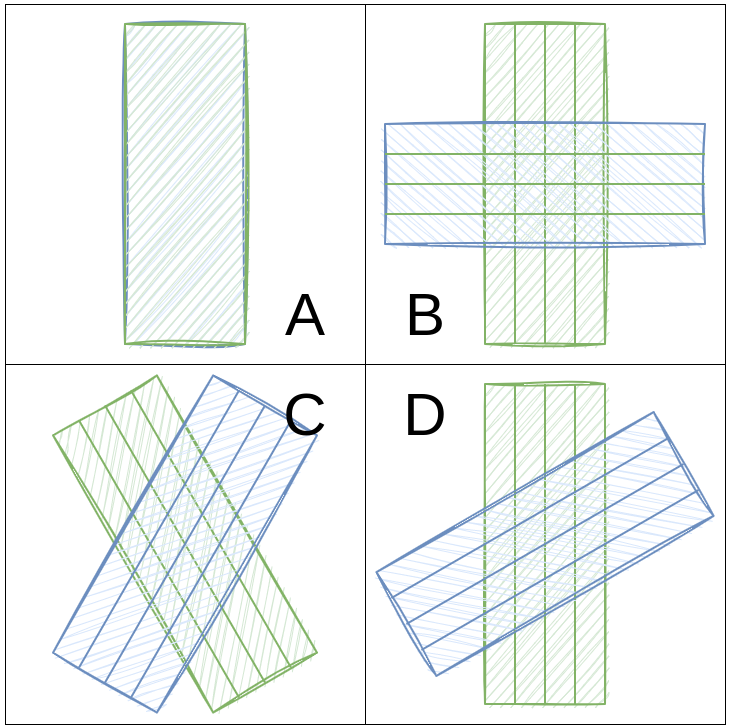
\includegraphics[width=0.41\textwidth, keepaspectratio]{Figures/muEDM/CyFi/CrossingFibres_config.png}
            \label{fig:CyFi:examples:a}}
            \subfloat[Projected uncertainties as a function of the outer layer's angle]{
            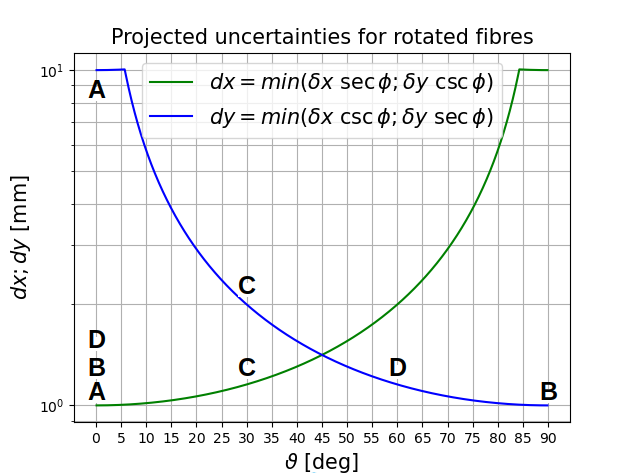
\includegraphics[width=0.57\textwidth, keepaspectratio]{Figures/muEDM/CyFi/projected_dxdy_examples.png}
            \label{fig:CyFi:examples:b}}
            \caption{Relation between the direction of the fibers and the associated uncertainties projected onto the axes. Some specific orientations of two overlapping ribbons are shown.}
        \end{figure}
        \begin{figure}
            \centering
            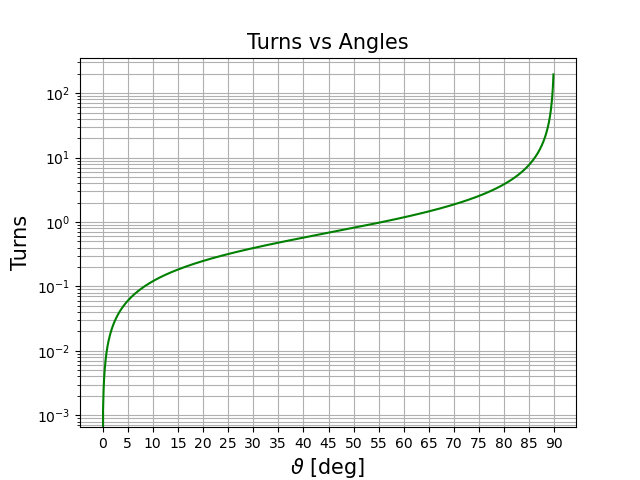
\includegraphics[width=\textwidth]{Figures/muEDM/CyFi/TurnsVsAngles.png}
            \caption{In a planar configuration, the angle at which the fibers run translates directly to the angle at which the ribbon is oriented. In a cylindrical geometry, a fiber running at a given angle will complete a different number of turns depending on the dimensions of the cylinder.}
            \label{fig:CyFi:TurnsVsAngles}
        \end{figure}
        \begin{figure}[ht]   
            \centering
            \subfloat[Projected uncertainties as a function of the outer layer's angle]{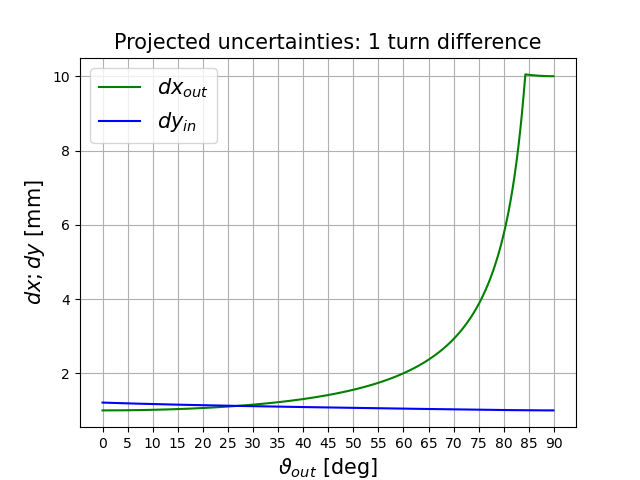
\includegraphics[width=0.49\textwidth, keepaspectratio]{Figures/muEDM/CyFi/projected_dxdy_1Turn.png}\label{fig:CyFi:projected_dxdy}}
            \hfill
            \subfloat[Angle of the inner layer and difference in angle as a function of the angle of the outer layer]{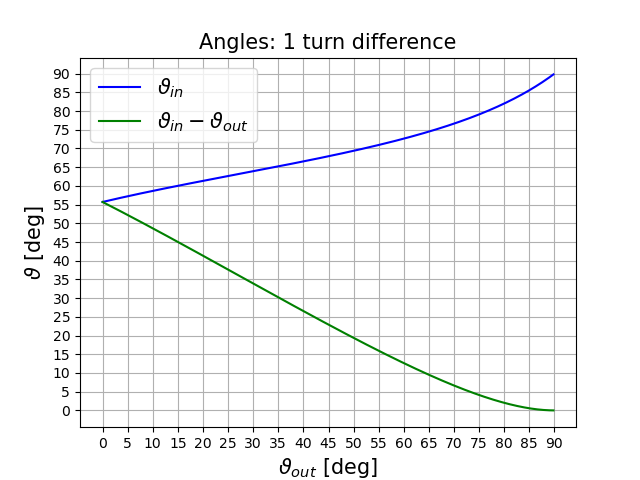
\includegraphics[width=0.49\textwidth, keepaspectratio]{Figures/muEDM/CyFi/Angles_1Turn.png}\label{fig:CyFi:angle}}
            \caption{The results when considering two layers in a cylindrical geometry keeping the requirement $\Delta T=1$: \ref{fig:CyFi:projected_dxdy} shows the projected uncertainties; \ref{fig:CyFi:angle} shows the angle of the inner layer.}
            \label{fig:CyFi}
        \end{figure}
        Building the layers with infinite precision on the angle is clearly not feasible for this reason we can use the plots in Fig.~\ref{fig:CyFi:5deg}, where the angles have been rounded to multiples of \SI{5}{\deg}. 
        Additional attention we can have is to consider the length of the scintillating fibers: if the fibers are too long the light collection at the ends is decreased by the absorption. The length of the fibers in both layers is shown as a function of the outer angle in Fig.~\ref{fig:CyFi:5deg:length}.
        Clearly, this is the extreme case: depending on the intrinsic resolutions of the fibers, shallower angles and $\Delta T<1$ could be chosen, simplifying the construction. \\
        The concepts here introduced are true for the system envisioned, but the specific values obtained depend on the specific dimensions of the cylinder as well as the intrinsic resolutions of a ribbon of fibers. 
        For the plots shown, we considered a cylinder of $r=\SI{3.1}{cm}$ and $h=\SI{20}{cm}$, reasonable sizes for the task at hand, and the intrinsic resolutions are here assumed $\delta_x = \SI{1}{mm};\ \delta_y = \SI{10}{mm}$.
        
        \begin{figure}[ht]   
            \centering
            \subfloat[Angle of the inner layer and difference in angle as a function of the angle of the outer layer]{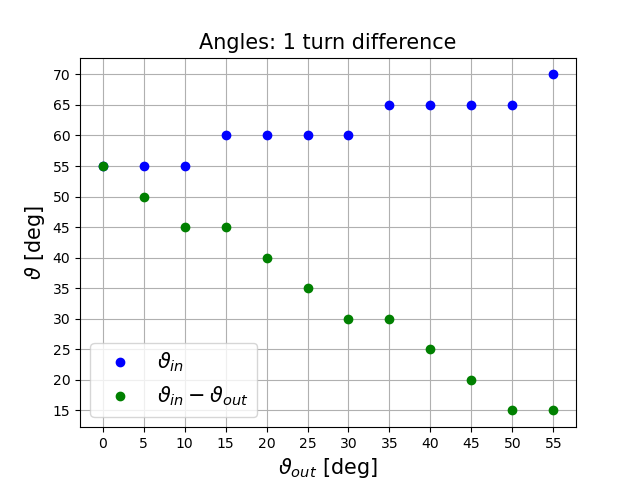
\includegraphics[width=0.49\textwidth, keepaspectratio]{Figures/muEDM/CyFi/Angles_1Turn_60deg_5deg.png}\label{fig:CyFi:5deg:angle}}
            \hfill
            \subfloat[Projected uncertainties as a function of the outer layer's angle]{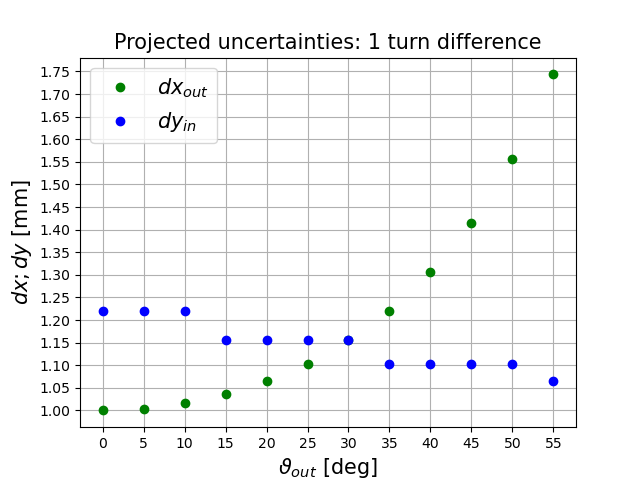
\includegraphics[width=0.49\textwidth, keepaspectratio]{Figures/muEDM/CyFi/projected_dxdy_1Turn_60deg_5deg.png}\label{fig:CyFi:5deg:projected_dxdy}}\\
            \subfloat[Fibers' length as a function of the outer layer's angle]{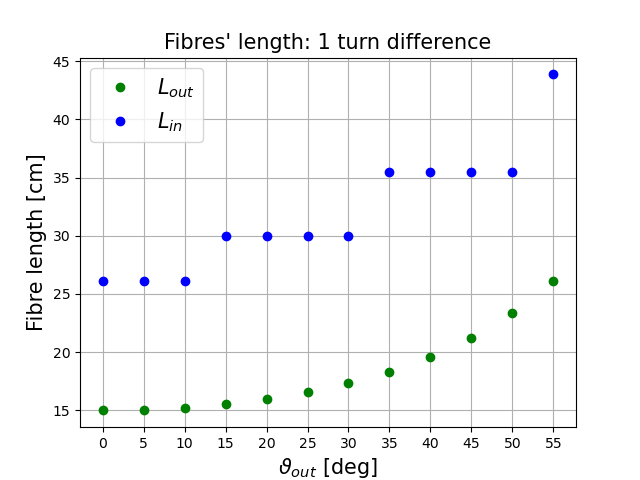
\includegraphics[width=0.49\textwidth, keepaspectratio]{Figures/muEDM/CyFi/FibreLength_1Turn_60deg_5deg.png}\label{fig:CyFi:5deg:length}}
            \caption{Key parameters as a function of the outer layer's angle keeping 1 turn difference between the two layers and rounding the angles to multiples of \SI{5}{\deg}.}
            \label{fig:CyFi:5deg}
        \end{figure}

    \status{started}
    \subsection{\gf simulation}
        The first hurdle in the Geant4 simulation for this sub-detector is the definition of the geometry.
        While the inside structure of the fibers and the readout are the same as discussed previously (see Sec.~\ref{}), the fiber shape is now less straightforward.
        
        \paragraph{G4TessellatedSolid}
        The shape is the result of wrapping a squared fiber around a cylinder resulting in a `squared helix'.
        After some consideration there are two ways of defying this geometry:
        \begin{outline}
            \1 Taking bool difference of two G4TwistedBox\footnote{The documentation can be found here: \href{https://apc.u-paris.fr/~franco/g4doxy/html/classG4TwistedBox.html}{G4TwistedBox}}. 
            This is a simple solution but comes with some limitations: the shape of the fiber cannot be changed to circular and the twisted box cannot be twisted more than \SI{90}{\deg}, so a stack of clones is needed; 
            \1 Defying the geometry using G4TessellatedSolid\footnote{The documentation can be found here: \href{https://apc.u-paris.fr/~franco/g4doxy/html/classG4TessellatedSolid.html}{G4TessellatedSolid}}, which means creating it by hand triangulating the shape. This is a more cumbersome solution but it allows for more flexibility.
        \end{outline}
        I decided to implement the latter to keep the possibility of simulating the detector with circular fibers.
        The core part of the code for generating the G4TessellatedSolid fibers, although perhaps not of particular interest, is in appendix \ref{ch:G4TessellatedSolid}.

        The resulting simulation, after having implemented everything so far described, is shown in Fig.~\ref{}.
        
    \status{review}
    \subsection{From $\upgamma$s to waveforms}
        The simulation in \gf ends with the recording of the optical photons entering the SiPM SensitiveDetectors.
        The physical processes going from the impinging photons to the analog signal are quite complex and simulating them would require a lot of effort (and CPU time).
        To get a feeling of the type of signals we can expect from the simulation we can create a simple script \textit{faking} the readout.
        The required steps are:
        \begin{outline}
            \1 \textit{PDF}: probability of a photon converting. 
            This is a binomial distribution and is SiPM dependent: reasonable values $p_{PDF}\in [0.3, 0.5]$
            \1 \textit{Response}: per photon converted, add a 'waveform' at the photon time. 
            The shape $w(t)$ is SiPM/electronics dependent but some assumptions can be made.
            \1 \textit{Dead time}: when a pixel generates a signal, any additional photon coming within a $t_D$ is lost.
            \1 \textit{Dark noise}: add a probability of spurious photons converting. 
            This is a Poissonian process that gives $n_{dark}$ photons distributed flat in the readout time.
        \end{outline}
        \begin{equation}
            W(t)=\sum_{i=0}^{n_\gamma} w(t_i|\Delta t>t_D)\cdot p_{PDF} + \sum_{i=0}^{n_{dark}} w(t_{flat}) 
        \end{equation}
        Once we obtain $W(t)$ we can apply a threshold $w_{th}$ and turn the signal from analog to digital. 
        If the $w_{th}$ is crossed, we recorded a \textit{hit}.
        In the geometry under consideration, a single particle crossing two fibers might generate 4 \textit{hits}, assuming reading the fibers at both ends.
        On top of this, the particle might generate scintillation in the neighbor fibers or some cross-talk might be present. 
        The general idea is to collect the signals from the fiber in each layer creating a 'layer'-\textit{hit} (a \textit{l-hit}). 
        This could then be combined to make a `cylinder'-\textit{hit} (a \textit{c-hit}).
        Mapping groups of hits in l/c-hits is not trivial and takes as parameters the dimensions of the cylinder and the SiPM numbers (or their position).

    \status{review}
    \subsection{Tracking}
    The details of the tracking procedure for the experiment are heavily dependent on the details of the detectors, which are not yet set in stone.
    The main option for a detector such as CHeT are
    \begin{outline}
        \1 To combine the \textit{hits} from the two layers in \textit{c-hits}. This would result in smaller uncertainties in \textit{xyz} but requires delicate handling of the correlation between the variables plus reduces the number of available hits. This would also cut the number of hits in half
        \1 To consider the \textit{hits} separately still in \textit{xyz}
        \1 To perform a transformation for the \textit{hits} in a more `natural' coordinate system: $xyz\ra r\varphi z$
    \end{outline}

    \paragraph{GENFIT}
        The tracking code could be developed from scratch or based on a pre-existing working code. 
        Given the size of the collaboration and the task, the second solution seems more adequate.
        In this regard, a good option would be to rely on a code developed for general track fitting in particle physics is GENFIT\footnote{\href{https://github.com/GenFit/GenFit}{GENFIT: https://github.com/GenFit/GenFit}}.
        %A brief description of the code itself can be found in App.~\ref{ch:genfit}.
        The development of the tracking procedure for the CHeT detector had to be put to a halt. This section is kept here just as food for thought for future development.

\status{started}
\section{A study of radial geometry}
    The development of the Pixel detector, supposed to be a counterpart to the CHeT, unfortunately, had some delay.
    This means that, during the first phase, the Pixel detector will not be available and the scintillating fibers need to be repurposed to be the only positron tracking detector.
    
\section{Conclusions}

\status{started}
\printbibliography[
    heading = bibliographychapter,
    title=Bibliography on muEDM positron tracker
]

\end{refsection}